\section{Kopplingsschema}

Nedan följer de kopplingsscheman som beskriver hur hårdvaran i Gloria hänger ihop.

\begin{figure}[h!]
	\centering
	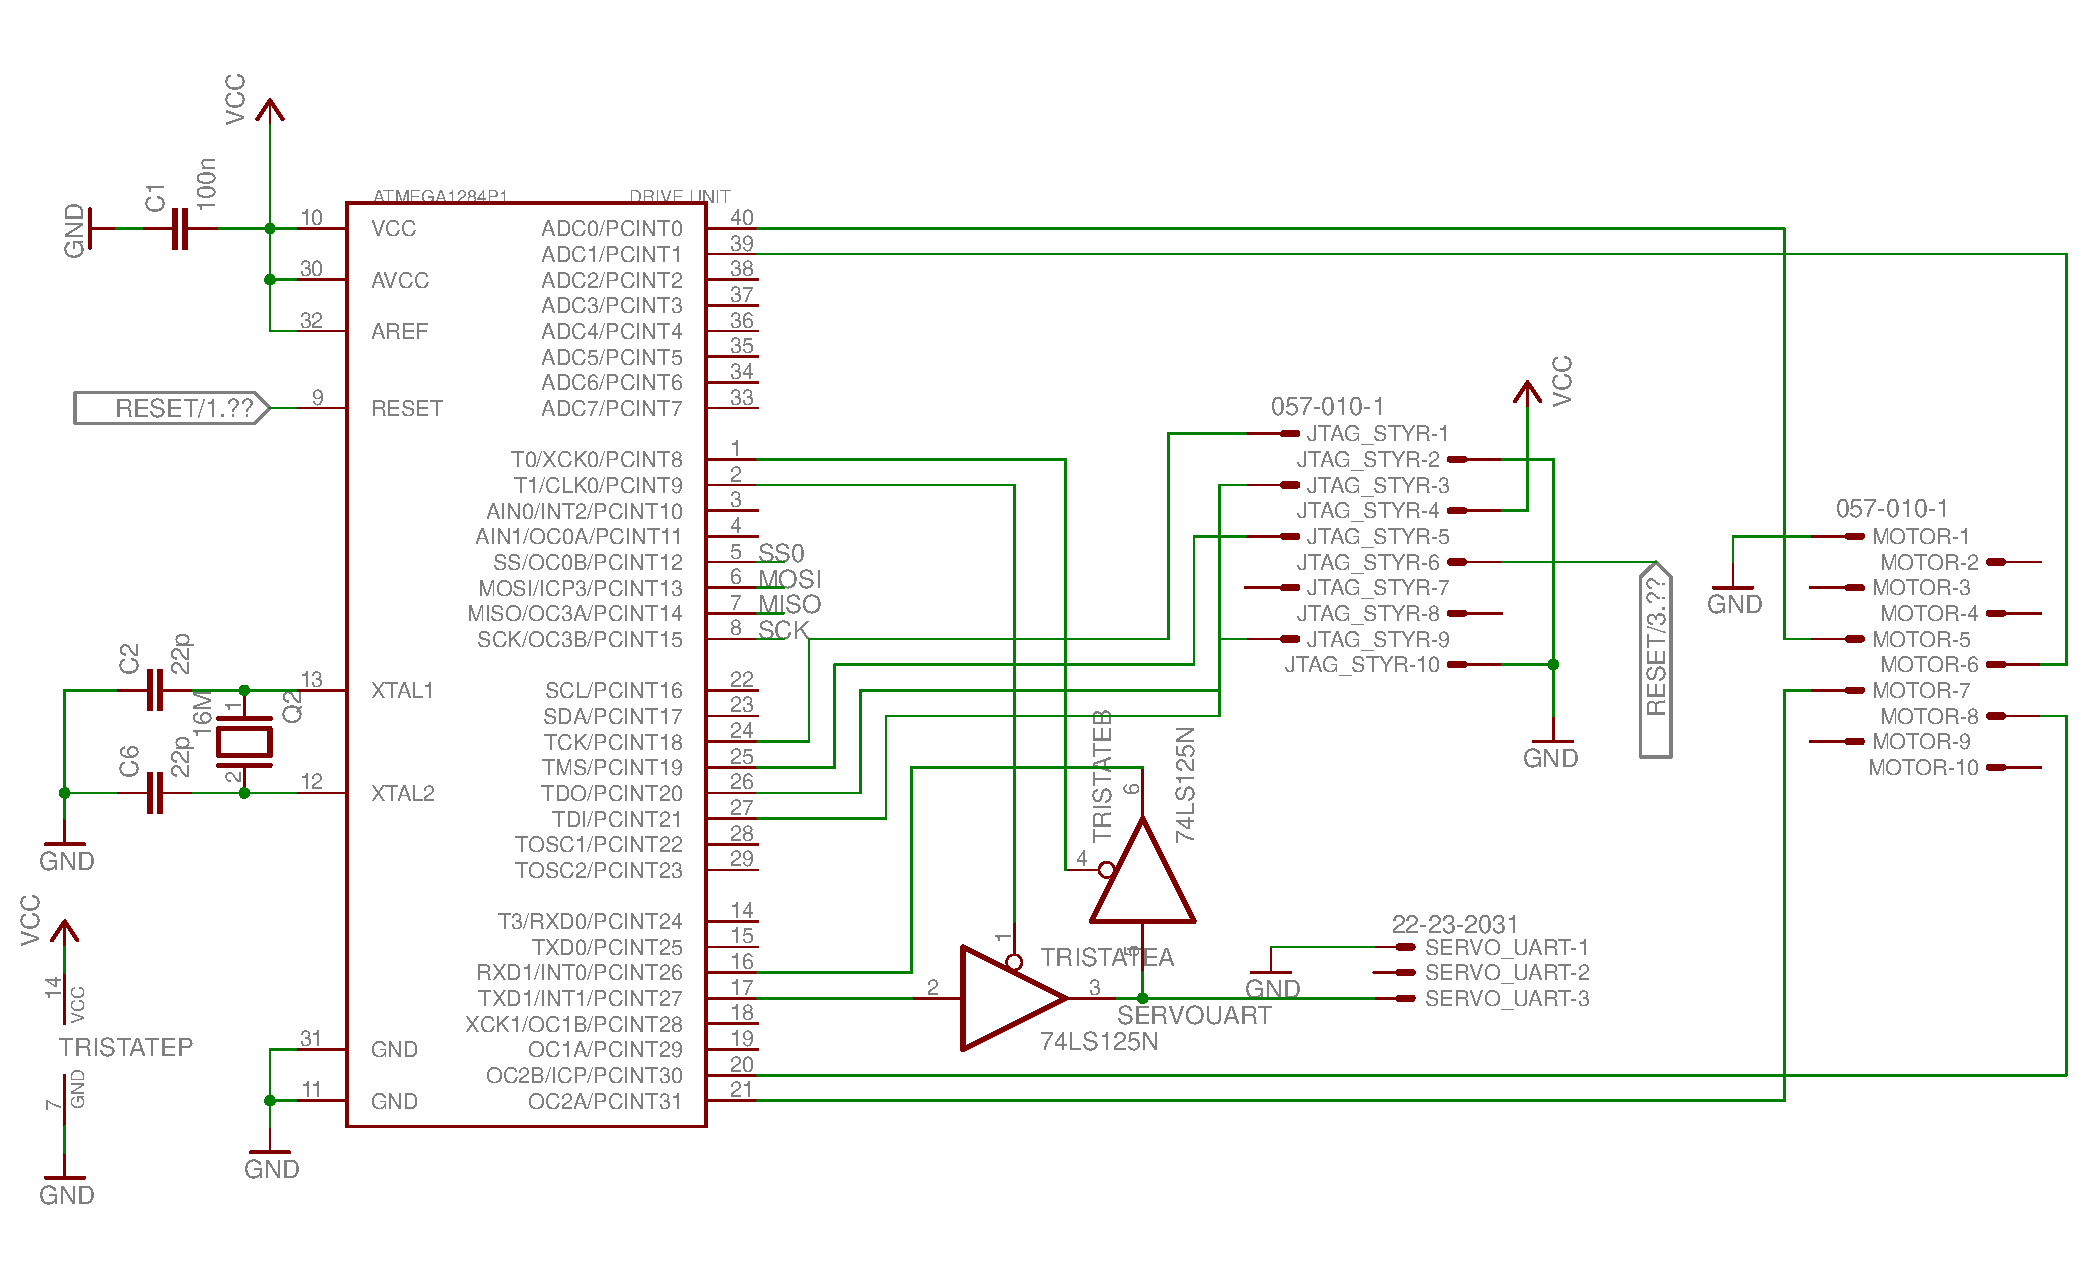
\includegraphics[scale=0.5]{grafik/kopplingsschema-drive_unit}
	\caption{Kopplingsschema styrenhet} \label{kopplingsschema-styrenhet}
\end{figure}

\begin{figure}[h!]
	\centering
	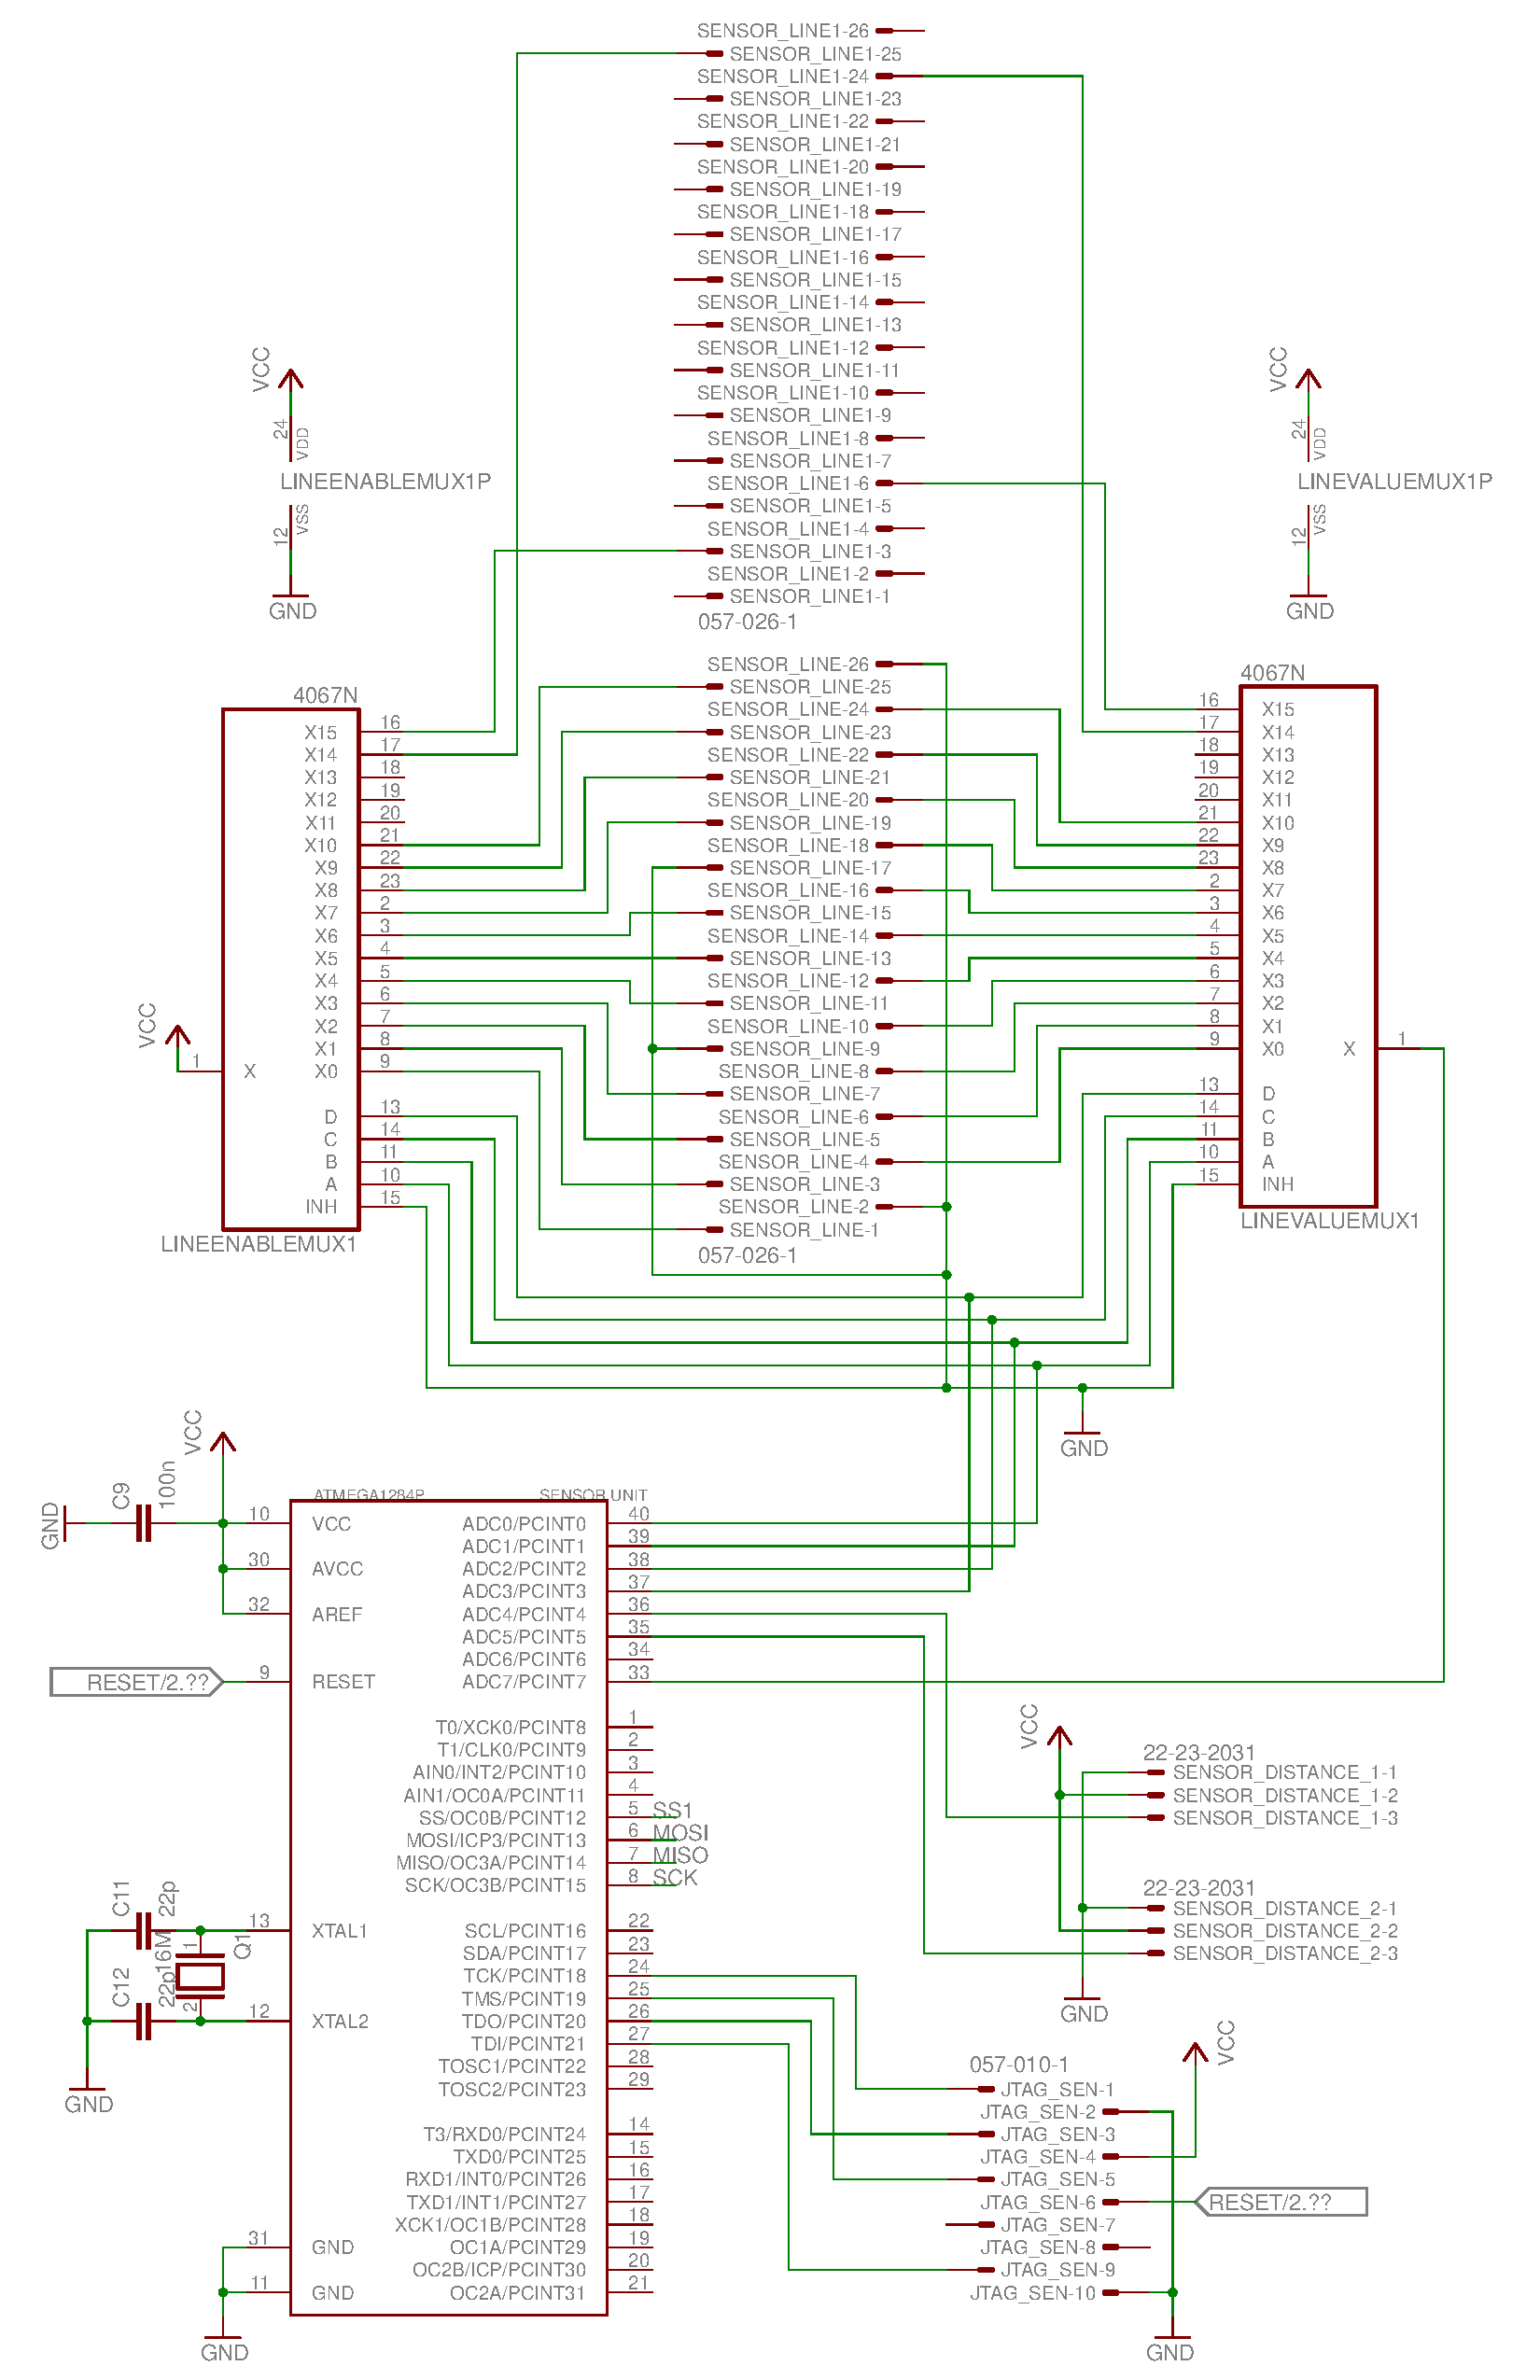
\includegraphics[scale=0.5]{grafik/kopplingsschema-sensor_unit}
	\caption{Kopplingsschema sensorenhet} \label{kopplingsschema-sensor}
\end{figure}

\begin{figure}[h!]
	\centering
	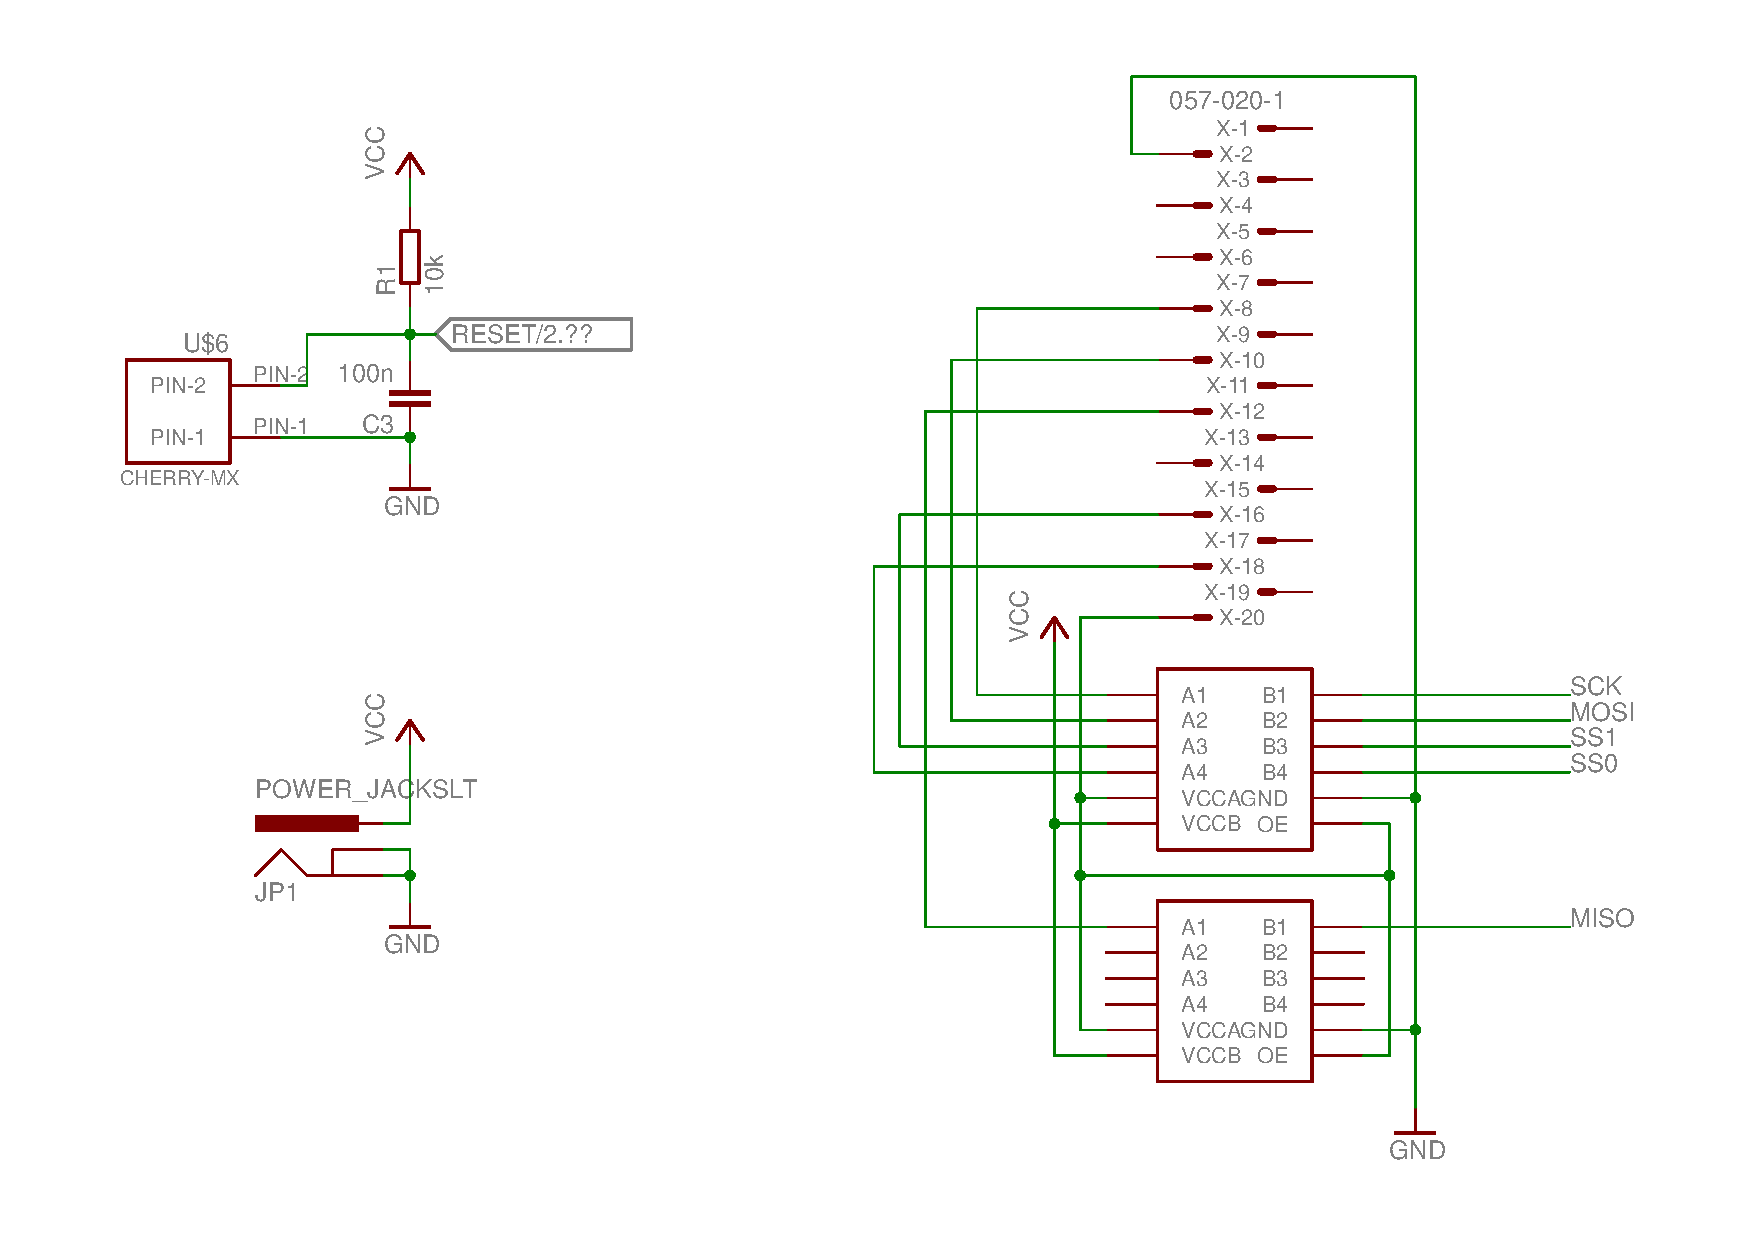
\includegraphics[scale=0.4]{grafik/kopplingsschema-level_shifters}
	\caption{Kopplingsschema level-shifters och reset-knapp} \label{kopplingsschema-levelshifter}
\end{figure}

\begin{figure}[h!]
	\centering
	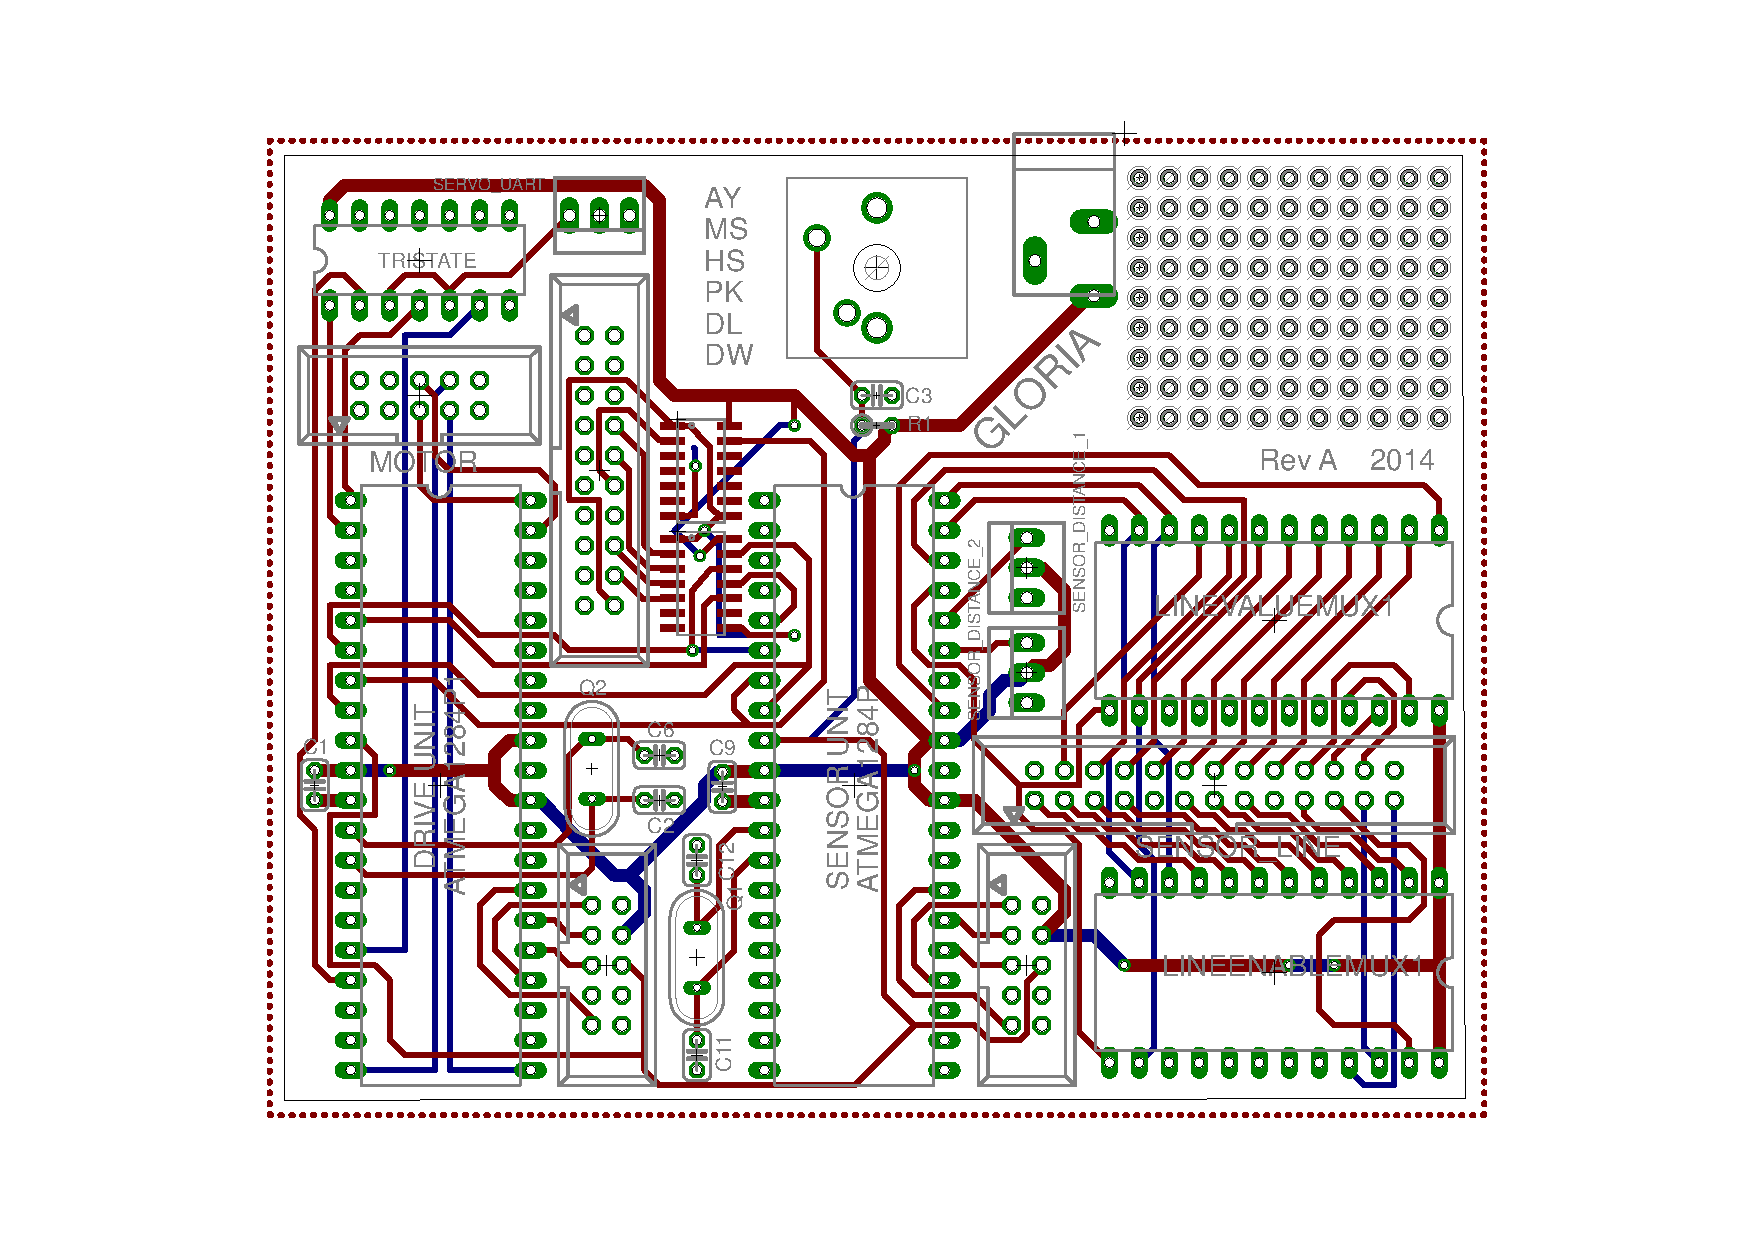
\includegraphics[scale=0.4]{grafik/kopplingsschema-pcb}
	\caption{Hur PCBn ser ut} \label{kopplingsschema-pcb}
\end{figure}
